%% LyX 1.3 created this file.  For more info, see http://www.lyx.org/.
%% Do not edit unless you really know what you are doing.
\documentclass[english]{article}
\usepackage[T1]{fontenc}
\usepackage[latin1]{inputenc}
\usepackage{graphicx}

\makeatletter
%%%%%%%%%%%%%%%%%%%%%%%%%%%%%% Textclass specific LaTeX commands.
 \newenvironment{lyxlist}[1]
   {\begin{list}{}
     {\settowidth{\labelwidth}{#1}
      \setlength{\leftmargin}{\labelwidth}
      \addtolength{\leftmargin}{\labelsep}
      \renewcommand{\makelabel}[1]{##1\hfil}}}
   {\end{list}}
 \newenvironment{lyxcode}
   {\begin{list}{}{
     \setlength{\rightmargin}{\leftmargin}
     \setlength{\listparindent}{0pt}% needed for AMS classes
     \raggedright
     \setlength{\itemsep}{0pt}
     \setlength{\parsep}{0pt}
     \normalfont\ttfamily}%
    \item[]}
   {\end{list}}

\usepackage{babel}
\makeatother
\begin{document}

\title{RGtk2 - A GUI Toolkit for R}

\maketitle

\section{Introduction}


\subsection{Motivation}

RGtk2 enables the R programmer to construct graphical user interfaces
with GTK+, a GUI toolkit that is very commonly used by linux desktop
applications and so is popular with the open-source community. The
R platform greatly benefits from access to GTK+ in that it allows
novice users, such as biologists, to capitalize on the analytical
functionality of R, without the hindrance of the learning curve associated
with a console-driven interface. For example, a graphical interface
could guide a biologist through a microarray data analysis task driven
by Bioconductor. GTK+ is a vast improvement over the existing GUI
toolkit for R, tcl/tk, as GTK+ is more advanced and, by virtue of
its popularity in open-source applications, is capable of integrating
interface functionality from a wide-range of other projects, including
GGobi and Mozilla Firefox.


\subsection{Background}

The original RGtk, based on the now obsolete GTK+ version 1.2, was
developed by Duncan Temple Lang. About 4 years ago, GTK+ 1.2 was overhauled
and renamed to GTK2. The fundamental GTK object system was abstracted
into a separate library called GObject, part of GLib. GTK2 also takes
advantage of the new font rendering library, Pango. Many widgets were
added, removed, and heavily altered. GTK2 has more sophisticated widgets,
prettier text, and a more elegant foundation than its predecessor.
RGtk2 is an attempt to catch up with the evolution of GTK+. The goal
is virtually complete support for the latest version of GTK2 (2.8.0)
and its underlying libraries.


\subsection{Scope}

GTK2 is dependent upon a collection of libraries, all of which RGtk2
aims to bind to R.

\begin{lyxlist}{00.00.0000}
\item [GLib:]Handles common tasks such as string manipulation, linked lists,
event looping, etc.
\item [GObject:]Contains object and dynamic type system, including properties
and signals.
\item [ATK:]Defines a common interface for accessibility technologies,
implemented by GTK.
\item [Cairo:]Vector graphics library with which GTK+ widgets are drawn.
\item [Pango:]Renders text, with full support for internationalization.
\item [GDK:]Handles interaction with native window system, including drawing
and events.
\item [GdkPixbuf:]Renders pixbufs, integrated with GDK.
\item [GTK:]Provides the widgets for the GUI.
\end{lyxlist}
Except for the first two, GLib and GObject, all of these libraries
are fully bound to R by RGtk2. GLib and GObject are partially bound
to the extent necessary for support of the others. A library binding
consists of several components:

\begin{lyxlist}{00.00.0000}
\item [Functions:]All functions are wrapped with automatic type conversion
of the parameters and return value(s). 
\item [Fields:]The values for fields of non-opaque structures are retrieved
and converted. This is read-only access.
\item [Callbacks:]User R functions are wrapped as typed C callback functions.
\item [Converters:]Library-specific types may require special conversion.
\end{lyxlist}

\section{Design}


\subsection{Goals}

The design goals of the project are two-fold. First, the bindings
must be complete and consistent with the bound API. This simplifies
documentation in that there is a more-or-less one-to-one correspondence
between RGtk functions and the API functions. This also ensures that
the R programmer has complete control over the API without any gaps
or deficiencies in functionality. Whatever the C programmer can do,
the R programmer should be able to do. Second, interaction with RGtk
must be simple and familiar to the R programmer. Foreign C concepts
such as memory management, return-by-reference parameters, and type
casting must be hidden or adapted to their R equivalent. The user
should be able to enjoy the benefits of GTK+ without knowing that
it is implemented in a foreign language.


\subsection{Central Problem}

Given the broad scope of the project, it is obvious that manual implementation
of the bindings would be extremely tedious and time consuming. In
order to avoid this, much of the code was autogenerated. Autogeneration
also enhances the maintainability of the project, since improved code
can be uniformly and automatically generated across all cases.

GTK+ and other GObject-based API's are defined according to a scheme-based
format called \emph{defs}. The definitions describe an API's object
hierarchy, function names, parameter types, structure fields, etc.
They are annotated with information that assists in more subtle aspects,
such as memory management. The most mature GTK+ language binding,
pygtk, maintains a set of reference \emph{defs} files and provides
python scripts for their generation and parsing. RGtk employs these
scripts for parsing the \emph{defs} files via RSPython. The result
is converted to R and C binding code through the use of a code generation
library implemented in R. The \emph{defs} format was overhauled along
with GTK+ in the transition to GTK2, and it contains much more information
than was provided to the original RGtk. However, there are still a
small number of functions that require manual implementation, such
as varargs functions and cases of complicated memory management.


\subsection{\emph{Defs} Shortcomings}

The annotated definitions are very helpful in generating code. Unfortunately,
the pygtk authors manually implement a large portion of their bindings,
so they rely less on the \emph{defs} information. The pygtk definitions,
therefore, are buggy and do not contain all of the information necessary
to come close to completely generating all of the bindings automatically.

The first task of building RGtk was the cleaning and annotating of
the \emph{defs} files. An example of an annotation is the specification
of a parameter as in, out, or in-out. This allows the code generator
to know when to accept a parameter as input to a function and when
to only return it as part of the result. Other additions include defining
explicit callback types for generating wrappers and specifying the
types of linked list elements, which is useful for type conversion.
Some of these modifications were not explicitly supported by the \emph{defs}
specification, but nor were they disallowed. The pygtk parsers were
extended to handle the new features, since they were written only
to handle the subset of the specification employed by the pygtk definitions. 


\subsection{Type Conversion}

Every component of the bindings requires type conversion to some extent.
The code generator attempts to write code that converts C types to
and from R. Primitive types, such as double {[}numeric{]}, int {[}integer{]},
and char{*} {[}character{]}, are perhaps the simplest to convert.
Opaque structures such as GObjects and {}``boxed'' types are passed
to R as externalptr's, with the class attribute set to a character
vector representing the type hierarchy of the object. Collections
of these types, in the form of arrays and linked lists, are simply
converted by iterating over the data structures. The original version
of RGtk supported this functionality, except for linked lists and
some array types.

A more complicated problem that RGtk2 attempts to solve is the conversion
of simple, transparent C structures that are normally initialized
manually and therefore lack a constructor. This problem could be solved
in at least two ways. First, a function could be added that serves
as a constructor for the structure. Unfortunately, this would break
the strict adherence to the API, since a new function is introduced.
Also, this solution violates the {}``spirit'' of the API's design.
The simple structures are meant to be initialized and manipulated
without the extra baggage of function calls. Given these disadvantages,
the alternative is favored: allowing the user to define an instance
of such a type as an R list which is automatically converted to the
corresponding C structure when passed to a wrapped function. When
an instance of such a type is returned from a function, it is converted
to its R list equivalent, preserving symmetry.

For example, suppose a user wished to construct an instance of GdkColor,
a structure describing an RGB color with fields red, green, and blue.
The following code would yield the color red: \emph{c(65535, 0, 0)}.
Here the fields for red, green, blue must be specified in the same
order as they occur in the C structure definition. If the user desires
an alternative order or does not wish to specify all of the fields
(they default to zero), then the list should be named according to
the field names in the C structure. For example, red could be specified
as \emph{c(red=65535)}.


\subsection{Memory Management}

Memory management in GObject-based libraries is based on the data
type. GObjects are reference counted, while boxed types are explicitly
freed after use. The memory persistence of other structures is either
freed on demand, based on reference counting, or is handled internally.
Finalizer functions for the boxed types are specified in the \emph{defs}.
The code generator registers these as the finalizers for the corresponding
externalptr in R. The reference counting of objects is also handled
automatically. Other structures may be special-cased in the generator
or dealt with manually. 

All of these mechanisms are dependent on whether RGtk {}``owns''
the memory of a returned value, which is also specified in the \emph{defs}
files. For example, if RGtk owns an object's memory, it does not need
to increase the reference count. If RGtk does not own an instance
of a boxed type, then it should not register its externalptr for finalization.
One shortcoming of the \emph{defs} format is that it is not possible
to specify the ownership of memory returned by reference, so these
cases must be dealt with using heuristics and manual implementation.


\subsection{Adapting to R}

Memory management is just one of the annoyances of C that R programmers
are happy to avoid. One example is the need to specify the lengths
of arrays (including strings) when passing them to functions, unless
it is assumed that the arrays are NULL-terminated. The code generator
uses heuristics to identify these parameters and does not require
R to provide them. The wrapping code determines the length of arrays
automatically. Another complication is the ability of C to return
values by reference. These parameters, in addition to the return value,
are returned to R compiled as a list. This avoids trying to emulate
the foreign concept of return-by-reference in R. As a final example,
certain errors that occur in GLib-based libraries are described by
a returned GError structure. In R, libraries often alert the user
to a problem via a printed warning. The RGtk2 user may specify whether
to print such a warning when a GError is returned by passing a parameter
to the wrapped function. If printing is not requested, the user can
still inspect the list structure containing the fields of the GError.


\section{Other Issues}


\subsection{The Event Loop}

Many GTK2 widgets have complex behavior that requires the execution
of timeout and idle tasks. In order to reliably invoke these tasks,
the GTK event loop must be the primary R event loop. The strategy
to achieve this depends on the platform. On Linux, the REventLoop
package by Duncan Temple Lang provides a framework for replacing the
default Read-Eval-Print Loop with a foreign loop, without losing control
of the console. RGtk2 provides a GTK2 (actually GLib 2.x) implementation
for the REventLoop package. On Windows, the solution is somewhat simpler.
The tcl/tk package invokes a function named \emph{tcl\_do} when it
is waiting for console input, so that it can still respond to tcl/tk
events. RGtk simply redefines \emph{tcl\_do} so that it checks for
GTK events instead. Both of these solutions are satisfactory, but
they are kind of ugly hacks.


\subsection{Compatibility}

The GTK+ API is in constant flux; it changes with each minor version.
RGtk must somehow accomodate the many different versions without overly
complicating the code generation process. For example, one solution
would be to autogenerate code with preprocessor directives allowing
conditional compilation based on the user's GTK version. However,
this would greatly complicate the process. It also would not account
for the R side of the wrappers. Instead, the RGtk code was simply
branched, so that as of this writing three minor versions of GTK are
supported (2.8.0, 2.6.0, and 2.4.0). As GTK and RGtk advance, the
previously branched versions will continue to be maintained by merging
version independent code enhancements between them. 


\section{Additional API Support}


\subsection{iWidgets}

Simon Urbanek's iWidgets is an attempt to establish a simple API for
quickly constructing GUI's in R. It is very minimalistic and thus
it should be relatively straightforward to provide iWidget implementations
based on any mature widget toolkit. In theory, it should allow the
R programmer to easily create a native GUI without concern for any
quirks or minutia associated with a particular platform or toolkit.
The programmer should be able to focus on the statistics without getting
bogged down in GUI building. RGtk2 provides a GTK2 implementation
of iWidgets, which is perhaps as close as one can get to native support
on Linux.


\subsection{Extra Libraries}

Two additional GTK-related libraries are included with RGtk2. The
first is libglade, which allows one to create a GUI by reading an
XML specification at runtime. The Glade graphical GUI builder exports
this XML, so even someone with little GUI programming experience can
quickly and easily construct a complex interface. Also, RGtk2 includes
GtkMozEmbed bindings for embedding a Mozilla Firefox renderer into
an RGtk2 application. This demonstrates the usefulness of binding
to a toolkit that is used by many major open source applications.


\section{Code Example / Demo}

The overall process of programming with GTK+ in R is essentially the
same as in C. Of course, in R there is no explicit memory management,
the syntax is a bit different, and R greatly facilitates many C chores.
An example is probably the best way to demonstrate how RGtk2 parallels
the C GTK+ API. The GTK+ distribution includes a demo of a simple
use of the {}``expander'' widget. 

The first step is to create a dialog to contain the widget (in C):

\begin{lyxcode}
window~=~gtk\_dialog\_new\_with\_buttons~(\char`\"{}GtkExpander\char`\"{},~NULL,~0,~

GTK\_STOCK\_CLOSE,~GTK\_RESPONSE\_NONE,~NULL);
\end{lyxcode}
In RGtk2's style, the function name, gtk\_dialog\_new\_with\_buttons
is collapsed to an easier to type gtkDialogNewWithButtons. The constant
stock item identifier is just given as its string value and the enum
GtkResponseType value is given as its equivalent string. This is a
var-args function, so C requires a NULL terminating argument, but
of course this is not necessary in R.

\begin{lyxcode}
window~<-~gtkDialogNewWithButtons(\char`\"{}GtkExpander\char`\"{},~NULL,~0,~\char`\"{}gtk-close\char`\"{},~\char`\"{}none\char`\"{})
\end{lyxcode}
Next, we want to make the dialog resizeable (in C):

\begin{lyxcode}
gtk\_window\_set\_resizable~(GTK\_WINDOW~(window),~FALSE);
\end{lyxcode}
For calling methods, RGtk2 supports a more convenient Java-like syntax
where the object is given first, followed by the \$ operator, then
the method and its arguments. Also note that in RGtk2, there is no
need to cast anything.

\begin{lyxcode}
window\$setResizable(FALSE)
\end{lyxcode}
Now it's time to set up a callback to the 'response' signal so that
we can close the dialog when the user is finished:

\begin{lyxcode}
g\_signal\_connect~(window,~\char`\"{}response\char`\"{},~G\_CALLBACK~(gtk\_widget\_destroy),~NULL);
\end{lyxcode}
RGtk2 supports an alias for g\_signal\_connect (connectSignal) to
save typing. It also takes advantage of R's convenience and lets you
leave off the unneeded user data parameter.

\begin{lyxcode}
connectSignal(window,~\char`\"{}response\char`\"{},~gtkWidgetDestroy)
\end{lyxcode}
Now we create a layout and add it to the dialog's internal layout
widget (vbox):

\begin{lyxcode}
vbox~=~gtk\_vbox\_new~(FALSE,~5);

gtk\_box\_pack\_start~(GTK\_BOX~(GTK\_DIALOG~(window)->vbox),~vbox,~TRUE,~TRUE,~0);
\end{lyxcode}
We need to access the 'vbox' field from R, so we use the '{[}{[}'
operator with the field's name:

\begin{lyxcode}
vbox~<-~gtkVBoxNew(FALSE,~5)

window{[}{[}\char`\"{}vbox\char`\"{}{]}{]}\$packStart(vbox,~TRUE,~TRUE,~0)
\end{lyxcode}
Here is the rest of the R code for the demo:

\begin{lyxcode}
vbox\$setBorderWidth(5)

label~<-~gtkLabelNew(\char`\"{}Expander~demo.~Click~on~the~triangle~for~details.\char`\"{})

vbox\$packStart(label,~FALSE,~FALSE,~0)\#~Create~the~expander

expander~<-~gtkExpanderNew(\char`\"{}Details\char`\"{})

vbox\$packStart(expander,~FALSE,~FALSE,~0)

label~<-~gtkLabelNew(\char`\"{}Details~can~be~shown~or~hidden.\char`\"{})

expander\$add(label)

window\$showAll()
\end{lyxcode}
Another reasonable introduction to the style and capabilities of RGtk2
is creating an R-based web browser using GtkMozEmbed, the embedded
Mozilla rendering widget.

The first step (after loading RGtk2) is to create our main window,
set its size and title, and then create the GtkMozEmbed widget. 

\begin{lyxcode}
browserWindow~<-~gtkWindowNew(\char`\"{}toplevel\char`\"{})

browserWindow\$setTitle(\char`\"{}RGtk~web~browser\char`\"{})

browserWindow\$setSizeRequest(800,~500)

mozembed~<-~gtkMozEmbedNew()
\end{lyxcode}
Next we need to define some user actions for the interface. The GTK+
API includes a convenience structure, GtkActionEntry, for quickly
defining and creating instances of GtkAction. The structure is an
example of a transparent type - we define it as a list in R. The action
group needs an array of actions, which means we combine the entries
in an R list, yielding a nested list structure.

\begin{lyxcode}
actionEntries~<-~list(

list(\char`\"{}BrowserBack\char`\"{},~\char`\"{}gtk-go-back\char`\"{},~\char`\"{}Go~\_Back\char`\"{},~\char`\"{}<control>B\char`\"{},

~~~~~\char`\"{}Go~back~to~previous~page\char`\"{},~browserBackward.handler),

list(\char`\"{}BrowserForward\char`\"{},~\char`\"{}gtk-go-forward\char`\"{},~\char`\"{}Go~\_Forward\char`\"{},~\char`\"{}<control>F\char`\"{},

~~~~~~\char`\"{}Go~forward~to~next~page\char`\"{},~browserForward.handler),

list(\char`\"{}BrowserRefresh\char`\"{},~\char`\"{}gtk-refresh\char`\"{},~\char`\"{}\_Refresh\char`\"{},~\char`\"{}<control>F\char`\"{},

~~~~~\char`\"{}Refresh~the~current~page\char`\"{},~browserRefresh.handler),

list(\char`\"{}BrowserHome\char`\"{},~\char`\"{}gtk-home\char`\"{},~\char`\"{}Go~\_Home\char`\"{},~\char`\"{}<control>H\char`\"{},

~~~~~\char`\"{}Go~back~to~initial~page\char`\"{},~browserHome.handler),

list(\char`\"{}BrowserStop\char`\"{},~\char`\"{}gtk-stop\char`\"{},~\char`\"{}\_Stop\char`\"{},~\char`\"{}<control>F\char`\"{},

~~~~~\char`\"{}Stop~operation\char`\"{},~browserStop.handler)

)

ag~<-~gtkActionGroupNew(\char`\"{}BrowserActions\char`\"{})

ag\$addActions(actionEntries,~mozembed)
\end{lyxcode}
The rest of the code necessary to create the browser may be found
as a demo in the RGtk2 package. There are many other demos available,
mostly converted from the C demos included with GTK+-2.0.

%
\begin{figure}

\caption{A screenshot of a web browser interface constructed from R, using
the GtkMozEmbed widget for rendering the HTML content. The navigation
buttons, URL entry, and statusbar are all driven by R callbacks.}

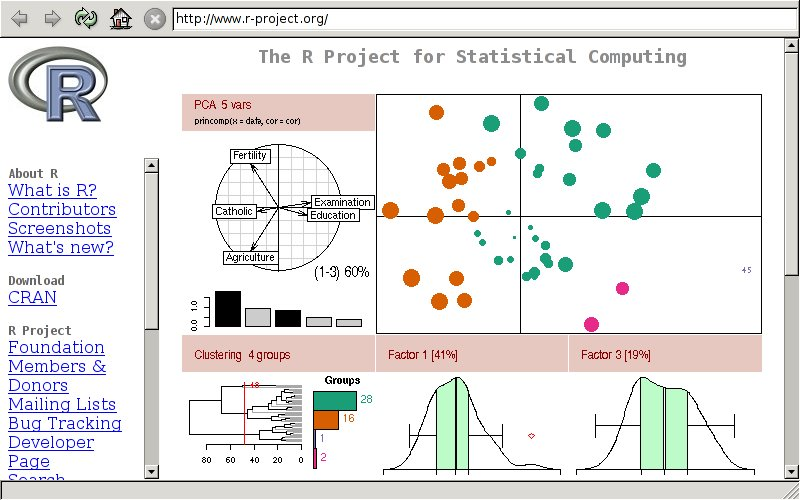
\includegraphics[%
  scale=0.5]{mozembed.jpg}
\end{figure}



\section{Conclusion}

In short, RGtk2 has achieved its goals of being complete and consistent
without sacrificing simplicity and familiarity to the R programmer.
A total of eight libraries are completely (and two more partially)
bound to R. Every attempt is made to keep a one-to-one correspondence
with the C API. Technologies such as glade and iWidgets greatly simplify
the task of creating GUI's using RGtk2. Finally, foreign C concepts
like memory management are avoided and assimilated, ensuring that
the learning curve for an R developer is as shallow as possible.

RGtk2 does, however, have several shortcomings, which hopefully will
be resolved in the near future. The maintenance of \emph{defs} files
is time-consuming and error-prone. Duncan Temple Lang is finishing
work on a new SWIG-inspired system for generating bindings directly
from C code. It promises to streamline the bindings generation process.
Another item on the wishlist is support for implementing new GObject
classes purely in R; however this would be a difficult task and the
great majority of RGtk-based projects would not benefit from it. Other
possible improvements include write support for structure fields (if
allowed), a cleaner event loop implementation (mostly depends on R
itself), and the ability to wrap varargs functions automatically.
Except for these improvements, most of the future work on RGtk2 will
be keeping up with additions to the GTK+ and related API's, ensuring
that the R developer is never left behind.

\begin{thebibliography}{99}

\bibitem{key-1}
The original RGtk: 
\emph{http://www.omegahat.org/RGtk}

\bibitem{key-3}
GTK+: 
\emph{http://www.gtk.org}

\bibitem{key-4}
R: 
\emph{http://www.r-project.org}

\bibitem{key-6}
GeneGobi: 
\emph{http://www.public.iastate.edu/~dicook/GeneGobi/MetNet_GeneGobi.htm}

\bibitem{key-7}
iWidgets: 
\emph{http://stats.math.uni-augsburg.de/R}

\end{thebibliography}

\end{document}
